
DBSCAN was developed by Martin Ester, Hans-Peter Kriegel, Jiirg Sander and Xiaowei Xu. All following definitions and descriptions are taken from their original publication \cite{dbscan} or their revisit of DBSCAN \cite{dbscanrevisited} and only apply to this algorithm.\\
Contrary to the aforementioned centroid-based partitioning algorithms (K-Means, K-Medoids and K-Medians) the DBSCAN (\textit{Density Based Spatial Clustering of Applications with Noise}) algorithm uses point densities to determine clusters.\\
To introduce the definition of the density of a cluster, first the Eps-neighbourhood of a point is defined:\\
\ \\
\textbf{Definition 1:} \textit{Eps-neighbourhood}\\
A point $q$ is part of the Eps-neighbourhood $N_{Eps}$ of point $p$ if the distance between them is smaller than or equal to a threshold distance called Eps.\\
The Eps-neighbourhood therefore is defined as $N_{Eps} = \{q \in D \ | \ ||p, q|| \leq Eps \}$ with $D$ denoting the entirety of points that are supposed to be clustered and $||p, q||$ being the distance between $p$ and $q$ for an arbitrary distance measure.\\
\ \\
The Eps-neighbourhood fails at being a reliable measure for the point density if a point is located at the border of a cluster. These points are called \textit{border points}. Points that are located on the inside of a cluster are called \textit{core points}. Hence the following definition is made:\\
\ \\
\textbf{Definition 2:} \textit{directly density-reachable and density-reachable}\\
A point $p$ is directly density-reachable from a point $q$ when
\begin{enumerate}
    \item $p \in N_{Eps}(q)$
    \item $|N_{Eps}(q)| \geq \text{MinPts}$
\end{enumerate}
with \acrshort{minPts} being the minimal number of points that $N_{eps}(q)$ should contain so that $q$ is considered a core point of a cluster.\\
A point is \textit{density-reachable} if there is a chain of points between $p$ and $q$ so that all neighbouring points in the chain are directly density-reachable.\\
\begin{figure}[H]
    \centering
    \subfloat[eps- neighbourhood]{{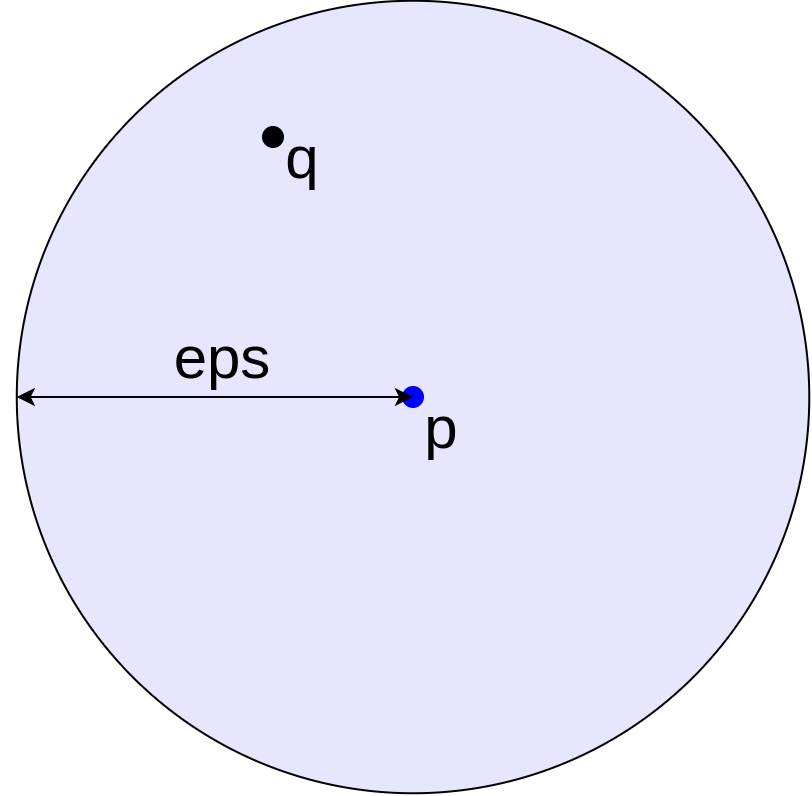
\includegraphics[height=7em]{./images/eps-neighbourhood}}}
    \qquad
    \subfloat[direct density-reachable]{{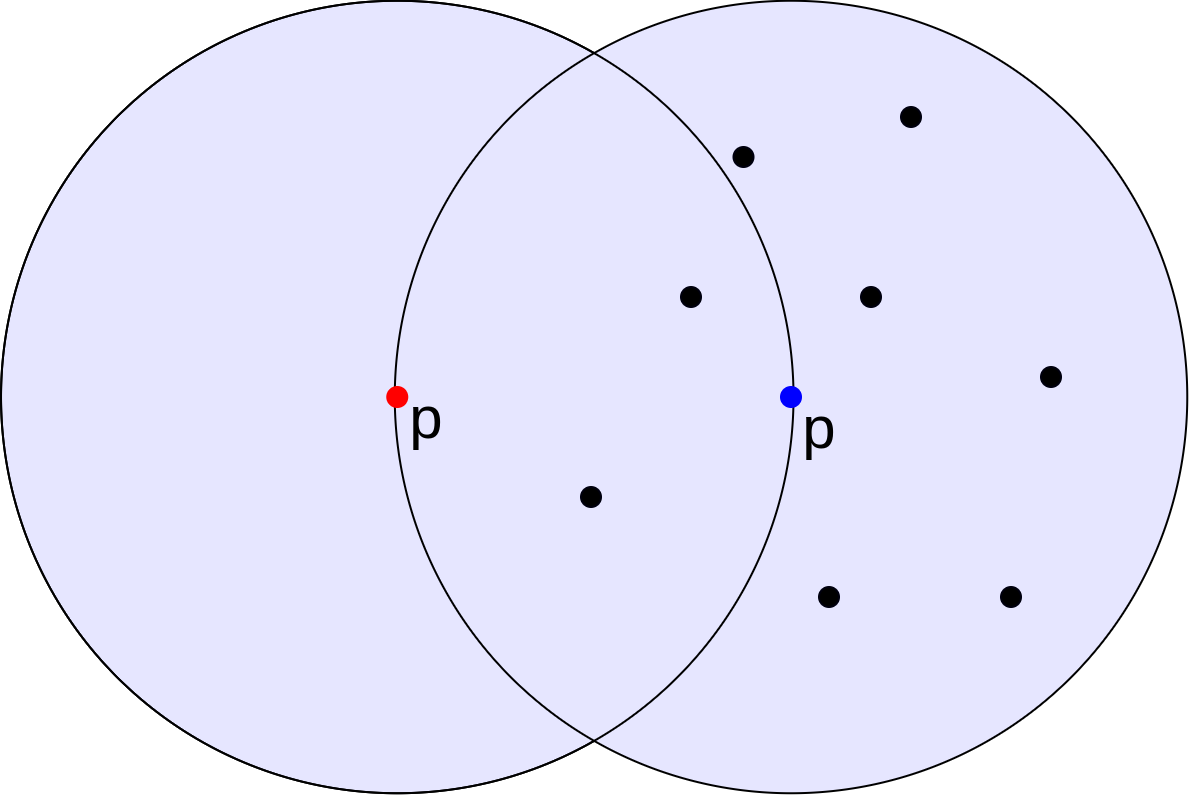
\includegraphics[height=7em]{./images/direct-density-reachable} }}
    \caption{visualisations of the definitions for eps-neighbourhood (left) and direct density-reachable (right)}
\end{figure}
To complete the definition of what is considered part of a cluster density-connectivity is defined:\\
\ \\
\textbf{Definition 3:} \textit{density-connected}\\
Two points $p$ and $q$ are considered density-connected if there is a common point $o$ which is density-reachable from $p$ and $q$.\\
\ \\
\begin{figure}[H]
    \subfloat[density-reachable]{{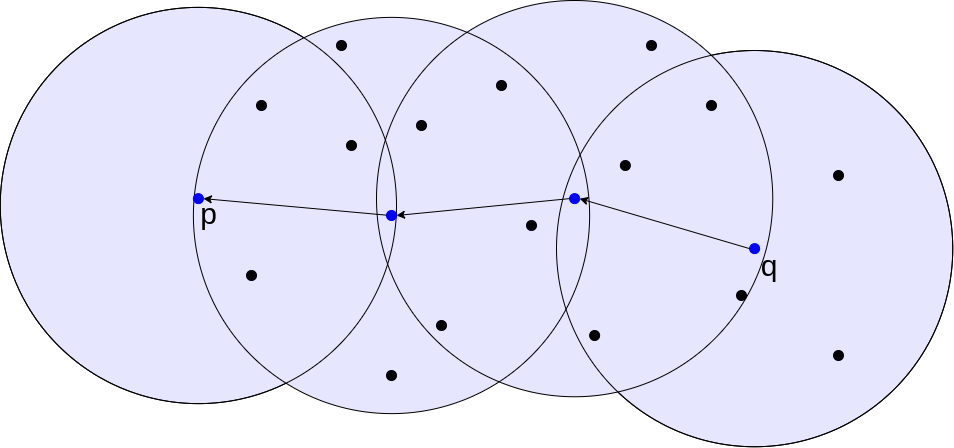
\includegraphics[height=7em]{./images/density-reachable} }}
    \subfloat[density-connected]{{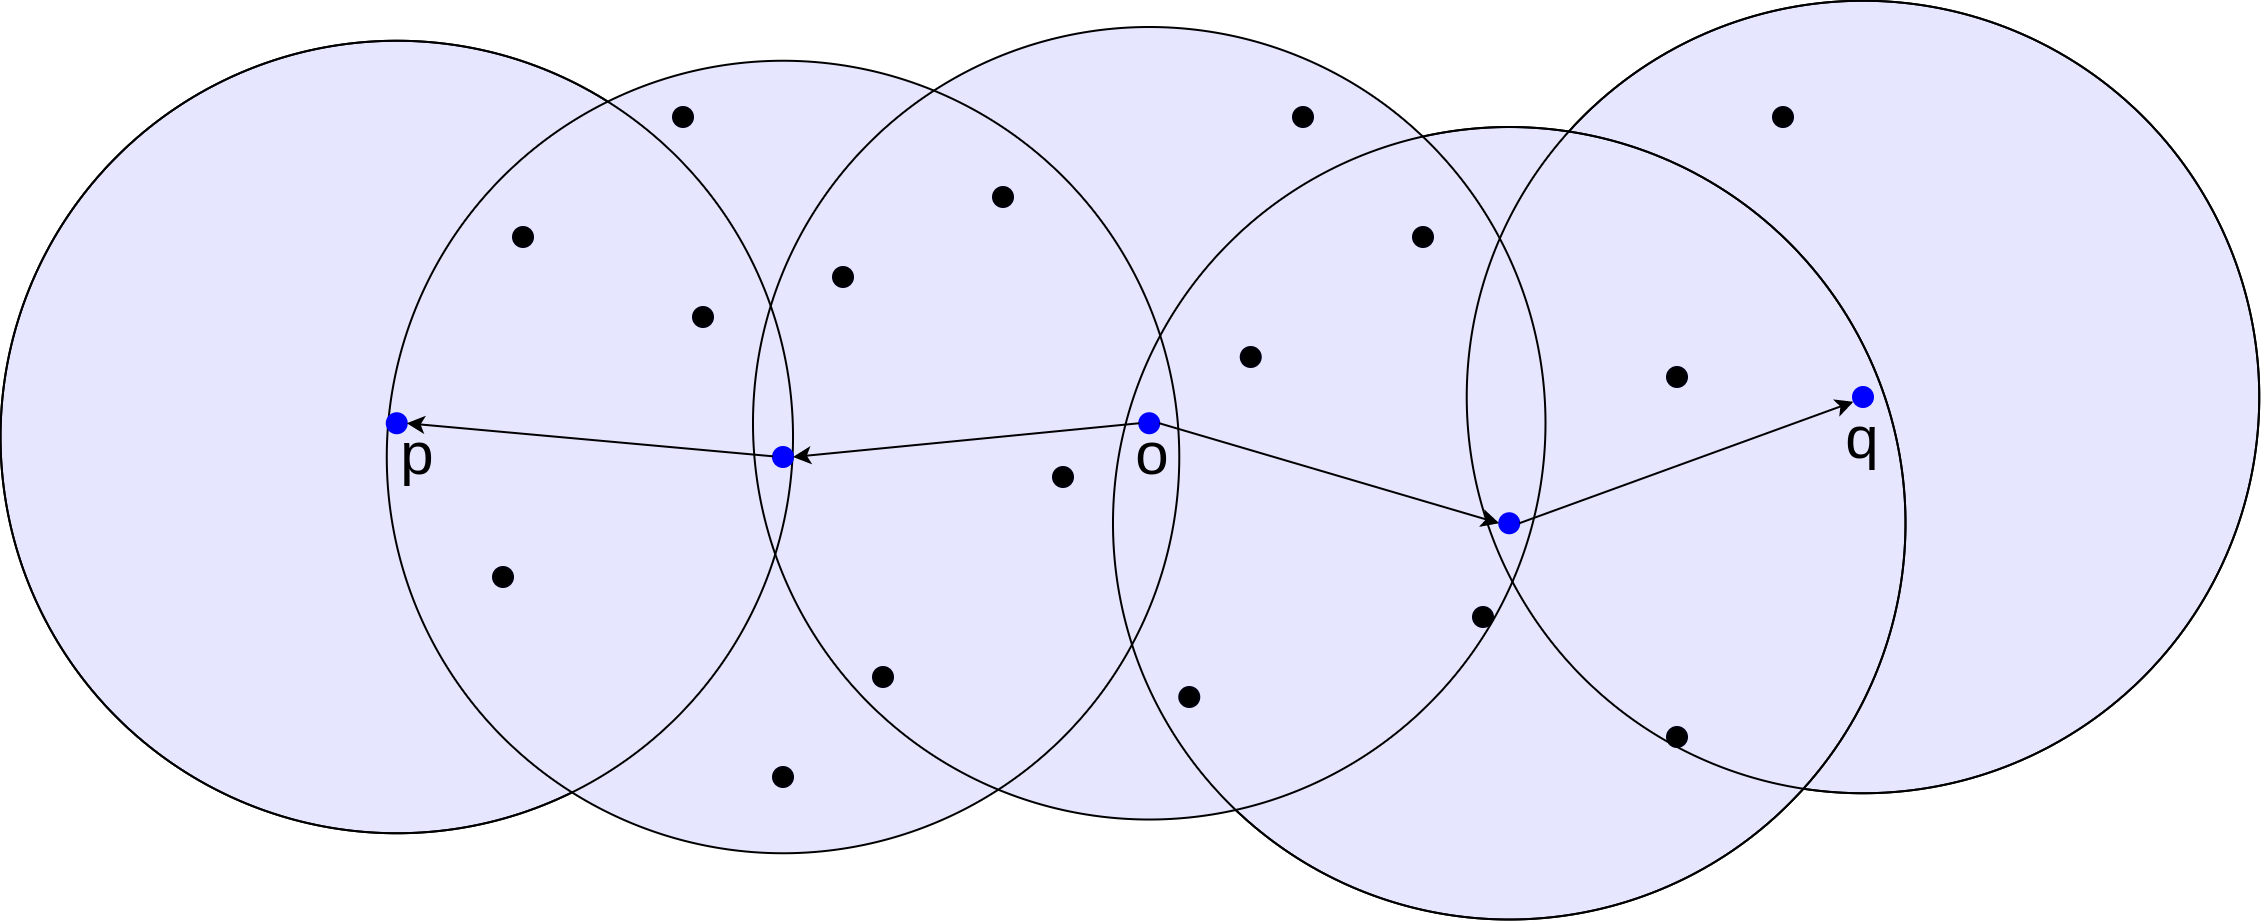
\includegraphics[height=7em]{./images/density-connected} }}  
    \caption{visualisations of the definitions for density-reachable (left) and density-connected (right)}
\end{figure}
Now a cluster can be described as:\\
\ \\
\textbf{Definition 4:} \textit{cluster and noise}\\
A cluster is a non empty subset $C \in D$ so that:
\begin{enumerate}
    \item $\forall p, q: p \in C \wedge q \text{ is density reachable from } p \Rightarrow q \in C$
    \item $\forall p, q \in C: \ p$ is density-connected to q
\end{enumerate}
\textit{Noise} is easily defined as every point that is not part of a Cluster $C_i$.\\
\ \\
Using these definitions DBSCAN can start the clustering process with given values for Eps and MinPts. First all points are marked as not labeled. Starting from an arbitrary point $p$ all points are iterated through in a linear fashion. For each point a \texttt{\Gls{glos:rangequery}} function is executed finding all directly density-reachable neighbours of $p$. If less then MinPts neighbours are found, $p$ is labeled as noise. Otherwise $p$ is a core point and is labeled as part of the currently explored cluster. If this is the case the neighbourhood of $p$, from now on denoted as S, is expanded.\\
\ \\
Unlabled points get checked for the core point condition (which equals a \texttt{RangeQuery} call) and all subsequent found neighbours are also added to S. Points that got labeled as noise beforehand and are part of S are labeled as part of the cluster.
When the expansion comes to an end a cluster is yielded, the next unlabeled point is chosen as $p$ and DBSCAN will continue to look for a new cluster.\\
\ \\
The biggest advantage of DBSCAN is its capability to find oddly shaped or spatially complex clusters. The aforementioned partitioning algorithms all fail at finding clusters that are not shaped like a sphere or a ellipsoid, if they are spatially entangled. scikit-learn published a great comparision of clustering algorithms on their website where the capabilities of DBSCAN are visualised \footnote{\url{https://scikit-learn.org/stable/auto_examples/cluster/plot_cluster_comparison.html}}. An example generated using the python script on the aforementioned site is shown in figure \ref{fig:dbscanadv}.

Moreover, DBSCAN allows for clustering without knowing the exact number of clusters or a termination criterion. Though finding the best values for minPts and eps can be equally challenging. The heuristic described in section \ref{dbscanheuristic} tries to simplify the estimation of these parameters.
\begin{figure}
    \centering
    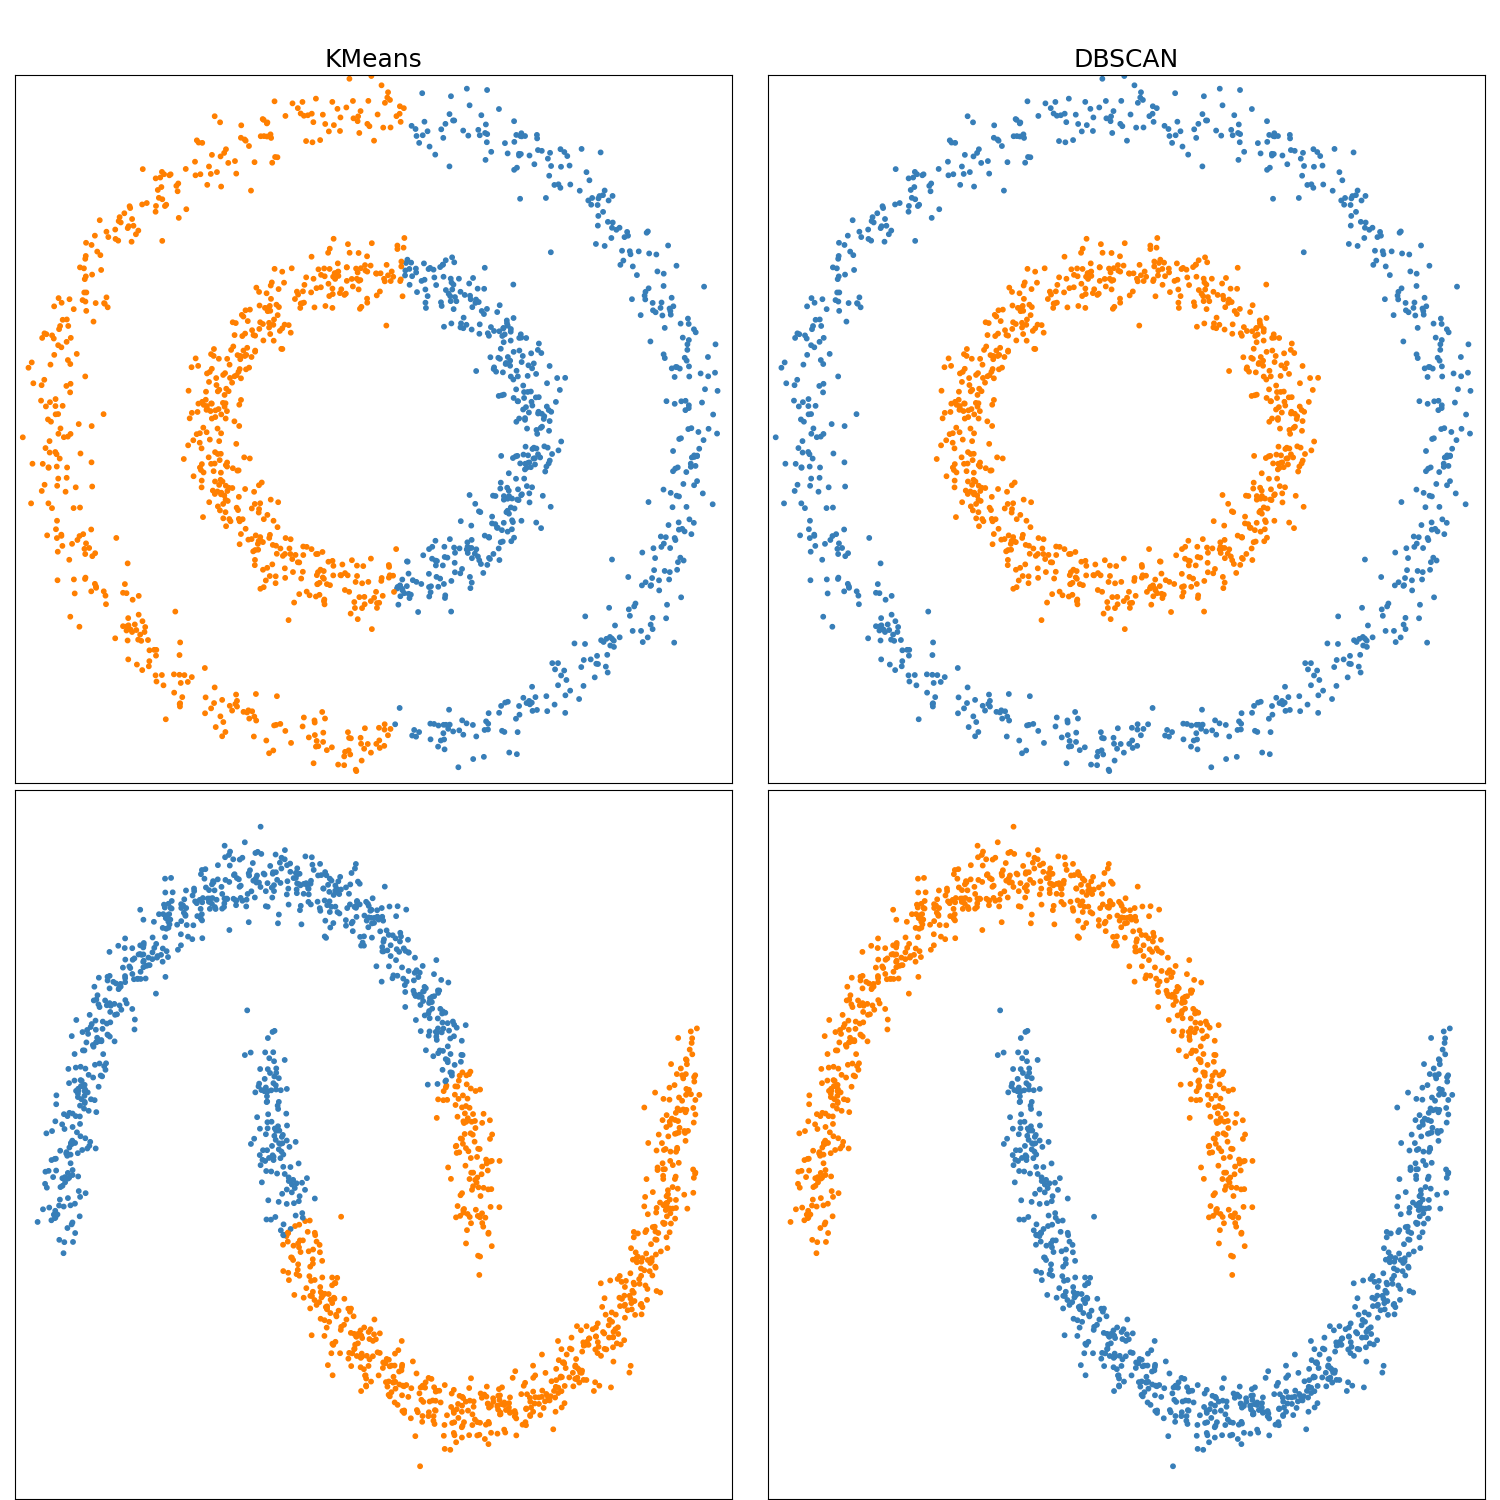
\includegraphics[width=0.4\textwidth]{../plots/dbscan/dbscan_comp}
    \caption{Comparision of DBSCAN to K-Means on spatially complex clusters}
    \label{fig:dbscanadv}
\end{figure}

Lastly, DBSCAN will fail at finding multiple clusters if they are spatially close to each other. Because of the nature of the Eps-neighbourhood all clusters with points seperated by a distance equal or less than eps can not be distinguished.

The runtime complexity of DBSCAN heavily depends on the runtime of the \texttt{RangeQuery} function which is executed for every point in the dataset once.
If \texttt{RangeQuery} is implemented using a linear scan, its complexity will be $\Theta (n \cdot D)$ with $D$ being the time needed for calculating the distance between points. Therefore the runtime complexity of DBSCAN is $\Theta(n^2 \cdot D)$ \cite{dbscanrevisited}.